\documentclass[a4paper,10pt]{article}
\usepackage[utf8]{inputenc}
\usepackage{graphicx}

%opening
\title{}
\author{}

\begin{document}

% \maketitle

\section*{Description of the General Archtecture}
\subsubsection*{mlsl\_parser}
The files \texttt{mlsl.waxeye} and \texttt{model.waxeye} contain the grammars for MLSL formulas and MLSL models.
We transform these grammars into the parsers \texttt{model\_parser.py} and \texttt{formula\_parser.py} with the parser generator waxeye.
The files \texttt{ast\_wrapper.py}, \texttt{model\_parser\_wrapper.py} and \texttt{formula\_parser\_wrapper.py} offer some helper functions to interact with the parsers generated by waxeye.

In \texttt{creae\_test\_formulas.py} we define functions to manually create syntax trees of formulas.
We use these trees in \texttt{test\_formula\_parser.py} to create test cases for the formula parser.

\subsubsection*{Main directory}
In the main directory we use \texttt{test\_sanity.py} and \texttt{test\_mc.py} for test cases and \texttt{model\_creator.py} to create models in those test cases.

\texttt{MLSL2Z3} transforms the model into a single instance of the class \texttt{View} and multiple instances of the class \texttt{Car}.
Then, \texttt{MLSL2Z3} transofrmes these instances into Z3 values.
Further, it transforms the syntax tree of the formula into Z3 cnstraints on these values.
Finally, it uses Z3 to determine if the constraints are satisfiable with the given values.
See Figure~\ref{fig:workflow} for a visualization.
\begin{figure}
	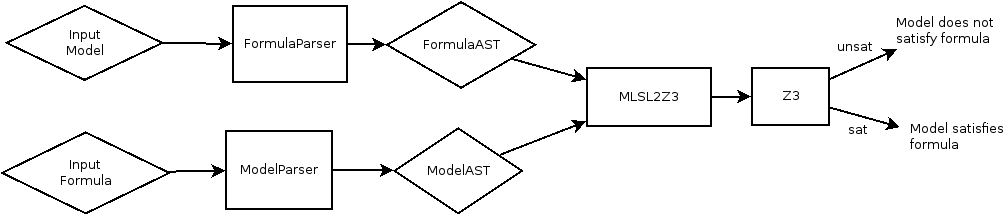
\includegraphics[scale=0.4]{workflow}
\caption{Workflow of \texttt{check\_static\_mlsl}.}
\label{fig:workflow}
\end{figure} 

The directory \texttt{lib} contains the libraries we use, i.e.\ Z3 and waxeye.

\end{document}
